\documentclass[openany,a4paper,12pt]{book}
\usepackage[utf8]{inputenc}
\usepackage{amssymb}
\usepackage{amsmath}
\usepackage{algorithm}
\usepackage{algpseudocode}
\usepackage{appendix}
\usepackage{tex/plugins/todonotes}
\usepackage{graphicx}
\usepackage{comment}
\usepackage{setspace}
\usepackage[
            backend=biber,
            bibstyle=numeric,
            doi=true,
            ]{biblatex}
\usepackage{booktabs}
\usepackage{fancyhdr}
\usepackage{pgfkeys}
\usepackage{pgfcalendar}
\usepackage{pgfgantt}
\usepackage{fancyhdr}
\usepackage{geometry}
\usepackage{listings}
\usepackage{float}
%Tikz-UML Dependancies - pdflscape used to fix landscape sections in pdf export
\usepackage{pdflscape}
\usepackage{tikz}
\usepackage{ifthen}
\usepackage{xstring}
\usepackage{calc}
\usepackage{pgfopts}
\usepackage[T1]{fontenc}
\usepackage{tex/plugins/tikz-uml}
\usepackage{pdfpages}
\usepackage[breaklinks=true]{hyperref}
\usepackage{breakcites}
\usepackage{microtype}
\usetikzlibrary{calc,trees,positioning,arrows,chains,shapes.geometric,%
  decorations.pathreplacing,decorations.pathmorphing,shapes,%
  matrix,shapes.symbols,math}


\onehalfspacing
% \renewcommand{\chaptername}{} % Remove chapter numbering
\bibliography{./bib/project.bib}

\title{Stigmergy for Multi-Robot Coverage}
\author{Michael Chadwick \\ ID: 200882675 \\ Professor Karl Tuyls}

\begin{document}
\maketitle
\tableofcontents

\thispagestyle{plain}
\begin{center}
    \textbf{Abstract}
\end{center} \label{dissAbstract}
A robotic swarm is composed of a large number of simple physical robots. From
the local interactions between the robots and the interactions of the robots
with the environment, an efficient global intelligence emerges. Multi-robot
coverage is the problem in which a swarm of robots needs to coordinate
decentralised in order to effectively and efficiently cover an unknown
environment.

The initial solution for the project involves using standalone posts, rope and
two large pieces of cloth.  By using the ropes in a similar manner to a boxing
ring, the solution provides flexibility in terms of arena size yet still 
contains the e-puck robots.

There has been previous attempts at this project, from the paper 'StiCo in
Action' \cite{Ranjbar-Sahraei2013Demo}.  The project is very similar in
that an implementation of the StiCo algorithm has been designed for both
projects, for the same robots.

For the robots, an implementation of the StiCo algorithm will be applied to
multiple e-Pucks for this project.  The program will be coded within the C
Programming language, and will utilise header files which define functionality
for the installed camera, wheels and LED lights whilst the source code will
handle the calling of said functionality, plus the image processing,
reading if there's a light trail ahead of the robot.

This project contains the source code for the StiCo algorithm, a stigmergic
methodology based on identifying a particular type of trail left by the agents
within a robotic swarm, and then moving away from said trails.

For some unknown reason, the IDE was unable to find the location of the header
files required within the program, meaning that the source code was unable to
be compiled, so I could not test the code upon 'live' robots.  Because of this,
I spent the time I had left in working with simulators - notably ENKI and
v-Rep \cite{enkiSite,vRepSite}.

I have used 'GitHub' as my method of storing my project \cite{GithubRepo}, as I
enjoy the portability granted to me and the ease of use it has given me whilst
interacting with this project.

\chapter{Introduction}
\section{Project Outline} \label{IntroOutline}
"A robotic swarm is composed of a large number of simple physical robots. From
the local interactions between the robots and the interactions of the robots
with the environment, an efficient global intelligence emerges. Multi-robot
coverage is the problem in which a swarm of robots needs to coordinate
decentralised in order to effectively and efficiently cover an unknown
environment. Examples include various monitoring, rescuing, and patrolling
scenarios. The purpose of this project is to set up an experimental
demonstrator, i.e. 'a dark room', in which multi-robot coverage experiments can
be conducted using e-puck robots, implementing the stigmergy principle as
observed in ant colonies. Ants use chemicals, called pheromones, to communicate
with each other via the environment. However, despite of a few reports of using
chemicals in robotic experiments, this is not a straightforward approach due to
difficulties in implementation and limited extendibility. Therefore, we take
advantage of a glow-in- the-dark foil (i.e. a foil covered by phosphorescent
material which absorbs UV light and re-emits the absorbed light at a lower
intensity for up to several minutes after the original excitation). As robots
need to emit light to the glow-in-the-dark foil, each e-puck robot is equipped
with a UV-LED pointing toward the floor. The glowing trails will take up the
role of natural pheromones."

\section{Problems Addressed by the Project} \label{IntroAddressed}
Primarily, the project helps to improve and refine the sharing of information
in conditions which may interfere with direct communication.  By indirectly
communicating, the robots no longer need large amounts of memory to store
the information, as it is held within the environment.  That way, the
information does not need to be stored for long periods of time on the robot,
only for enough time to process what the information means to the robot.

As mentioned in the Project Outline \ref{IntroOutline}, some of the
applications include travelling in potentially uncharted territory, or in
dangerous situations such as searching for explosives whilst patrolling.
There are other fields which this project could benefit from, too.  Some
examples could include the medical profession in surgery, by having machinery
following the lines drawn on patients instead of staying away from the
localised information.  Another potential use could be within biology.  As this
project aims to emulate some of the functional methods that animals have,
successfully doing so can help us to document and understand reasons for the
evolutionary choices that were made for the species.  This project itself does
not focus on these potential applications - instead it is the functionality and
implementation of an aspect that some animals possess.

\section{Aims and Objectives of the Project} \label{IntroAims}
Project aims include coding an implementation of a stigmergic algorithm for the
'e-puck' hardware platform, which will utilise the use of glow-in-the-dark
materials as the method of storing the localised information and processing the
data in such a way that it allows for a uniform spread of entities across an
area.  Plans for an area are also included within the scope, so that
researchers have a basic platform for testing created algorithms.

\section{Challenges within the Project} \label{IntroChallenges}
There are a couple of challenges that this project has that are inherent to the
subjects that link together as a part of the project.  As with anything which
has robotics as it's main focus, it can be difficult to produce workable source
code, as the platform you are writing for is different to the target
architecture, more often than not, and have specific Application Programming
Interfaces (APIs) which need to be utilised.

Another hurdle to overcome for this project would be how the robots are
required to have some form of autonomy.  As their reactions are based on the
environment, meaning that each iteration can have a slightly different outcome,
depending on the criteria.  In larger projects, this can make testing difficult
and time-consuming.

There are also challenges which affect all projects.  Potential risks such as
time management, disorganisation and ambiguity all play a role within the 
final outcome of the project.

\section{The Produced Solution} \label{IntroProducedSolution}
This project contains the source code for an implementation of the StiCo
algorithm, a stigmergic methodology based on identifying a particular type of
trail left by the agents within a robotic swarm, and then moving away from said
trails.  This allows the agents to spread across an area in a uniform fashion,
with each robot focusing on a particular area.  There are also some schematics
for a proposed arena to hold the robots, allowing a testing ground to be built.

\section{The Project's Success} \label{IntroSuccess}
Unfortunately, as a generalisation, the project would be deemed a failure.
The 'Challenges within the Project' \ref{IntroChallenges} section lists an
overview for the reasons as to the cause - more detail will be given throughout
this document.

\chapter{Background}
\section{Background of the Project}
%Who the project is being done for (your supervisor, and any external customer);
The project is being completed for Professor Karl Tuyls in the
department of Computer Science, University of Liverpool.
The Project is also applicable for anyone wishing to build an area in which to
conduct simulations that utilise the E-Puck platform\cite{ePuckSite}.

%What the proposed solution is, how the aim will be achieved.
The initial solution for the project involves using standalone posts, rope and
two large pieces of cloth.  By using the ropes in a similar manner to a boxing
ring, the solution provides flexibility in terms of arena size yet still 
contains the e-puck robots.  The posts will hold up the large pieces of cloth
--- a darker throw for the internal ceiling of the arena, and a lighter cloth
for the theoretical 'roof' of the structure.  The paler cloth reflects most 
external light which would otherwise cover the sectioned
area; the darker colour absorbs light within the structure.

With this solution the size of the area can be modified thanks to the rope.
The dual-layered cover prevents most light from entering the area.
Openings that may be made within the lower layer of fabric would allow
visual monitoring with little compromise.

There are multiple research papers on decentralised robots --- for patrolling,
there is the Edge Ant Walk (EAW) algorithm, which V. Yanovski has worked on
\cite{Yanovski2003}.  Due to memory limitations, the demonstration will be 
the StiCo\cite{Ranjbar-Sahraei2012} as well as the work on HybaCo
\cite{Broecker2015}.  Research into Robotic implementations of pheromone-using
insects will be the main area of
research\cite{Yanovski2003,Ranjbar-Sahraei2012,Broecker2015}.
Tangentially relevant information includes looking into Auction-based
methods of sharing tasks\cite{Schneider2015}.

\section{Existing Solutions}
There has been previous attempts at this project, from the paper 'StiCo in
Action' \cite{Ranjbar-Sahraei2013Demo}.  The project is very similar in
that an implementation of the StiCo algorithm has been designed for both
projects, for the same robots.

There are also variations on the robot that you can use for this test.  It
could be possible to use a Raspberry Pi \cite{raspberryPiSite} with it's
camera attachment as a base for custom made robots.

There's also multiple emulators for the e-puck robot, so the information can
be simulated in the circumstance that you do not have enough robots at the
time, or if it would be inefficient to test with the higher quantities of
robots.  From the simulators listed \cite{ePuckSiteSimulators}, during the
project I have attempted to test 'ENKI' (\cite{enkiSite}) as well as 'v-Rep'
\cite{vRepSite}.  Whilst I was happy with the concept of Enki, I could not
find out enough from the documentation to compile and test my code within this
simulator.  V-Rep, on the other hand, had a lot of information show initially
and I have included some images which show my progress.

\section{Relevant Research}
Information which has been of use within this project would be the website and
documentation of the robotic platform known as the 'e-Puck'
\cite{ePuckSite}, as it was the target platform for the project.  This robot
is ideal as it has the requirements for the project - a light, camera and 
propulsion.  The robot can be controlled externally via Blue-tooth as well as
running a program.

Similar theories, such as the BeePCo and HybaCo algorithms
have also been heavily relevant within the process of this project
\cite{Broecker2015Demo,Caliskanelli2015,Lemmens2008}, and have been used as a
form of unofficial evaluation throughout the project as well as a valuable
source of information in the theory, and it's application, of robotics-based
projects.

There was a lot of programs which I have had little to no experience in using,
which were utilised within the project.  A main example would be the notion
of coding for a platform you are not writing your source code upon.
Personal preference is to code using simpler editors and without large
development environments with multiple perspectives on the source code.  Whilst
much has been realised, my preference still holds.  Another section of software
that was utilised during the project which required research was the
simulators, as I had no prior experience in emulating robotics.

As part of the project, an arena and it's blueprints were erected to test the
concept of using rope as the edges of an arena - reducing the amount of heavy
parts and making a smaller storage footprint.  For this, I had learnt a basic
knot which helps to hold the rope together and increase it's rigidity in
between the connected posts.

\section{Project Requirements}
%What the aim of the project is, what it is intended to achieve;
Project Aims include building the testing grounds for the robotic simulations as
well as showing a demonstration of the arena through the use of the e-Puck
hardware platform.  With the completion of this project, researchers have the
capability of producing a testing ground for their experiments with the e-Puck
hardware platform.  The demonstrative section aims to show that the arena is
capable and performs it's required task.

For the robots, an implementation of the StiCo algorithm will be applied to
multiple e-Pucks for this project.  The program will be coded within the C
Programming language, and will utilise header files which define functionality
for the installed camera, wheels and LED lights whilst the source code will
handle the calling of said functionality, plus the image processing,
reading if there's a light trail ahead of the robot.

\chapter{Data Required}
\section{Data Used within the Project} \label{DataDefined}
Apart from research purposes, there has been little data used within this
project.  The StiCo algorithm pseudo code was taken from the 'Stigmergic
Coverage Algorithm for Multi-Robot Systems (Demonstration)' paper
\cite{Ranjbar-Sahraei2012Demo}.  For the introductory stages (Designing the
solution, defining the Project Requirements), this was the only information
used in a fashion outside of citation or referencing.

During the implementation stage, I have been looking through the available
sample code which was obtained from the 'GCtronic Wikipedia website'
\cite{gCtronicEpuckSite} as a base of understanding when it came to coding
the StiCo Algorithm.  I have also simulated some tests whilst I was
building the source code for the e-Puck robots.

Tangentially related data throughout the project includes documentation on the
various pieces of software I have used throughout this project.  An incomplete
list would include the text editors and IDEs that I have used (Vim, MPLAB X,
TeXstudio) as well as the simulation programs for the e-puck Robot (ENKI,
v-Rep).

\section{Ethical use of Data} \label{DataEthics}
To the author's knowledge, only synthetic data has been used within this
project, which is the information created by the author, for the sole purpose
being this project.  Whilst source code has been examined during this project
with the purpose of understanding coding concepts that are unfamiliar, along
with previously made header files as part of controlling the robot (in terms of
firmware), nothing has been knowingly taken without required authorisation.
The firmware used is currently included within the project's repository 
\cite{GithubRepo} for the sake of completeness and compatibility.
There has been no data which has been used within this project that is outside
of what has been defined within this chapter.

\section{Ethical use of Participants} \label{DataParticipants}
There have been no official participants within this project.  Whilst the
author has unofficially discussed potential options in completing this project
with colleagues and superiors during times of leisure, for the sake of
obtaining their opinion in the author's progress, there have been no
collaborators in designing, building or testing for the project.

\chapter{Design}
\section{Summary of Proposal}          \label{desProSum}
%Statement of background, aims and objectives
\subsection{Project Outline} \label{desProOut}
"A robotic swarm is composed of a large number of simple physical robots. From
the local interactions between the robots and the interactions of the robots
with the environment, an efficient global intelligence emerges. Multi-robot
coverage is the problem in which a swarm of robots needs to coordinate
decentralised in order to effectively and efficiently cover an unknown
environment. Examples include various monitoring, rescuing, and patrolling
scenarios. The purpose of this project is to set up an experimental
demonstrator, i.e. 'a dark room', in which multi-robot coverage experiments can
be conducted using e-puck robots, implementing the stigmergy principle as
observed in ant colonies. Ants use chemicals, called pheromones, to communicate
with each other via the environment. However, despite of a few reports of using
chemicals in robotic experiments, this is not a straightforward approach due to
difficulties in implementation and limited extendability. Therefore, we take
advantage of a glow-in- the-dark foil (i.e. a foil covered by phosphorescent
material which absorbs UV light and re-emits the absorbed light at a lower
intensity for up to several minutes after the original excitation). As robots
need to emit light to the glow-in-the-dark foil, each e-puck robot is equipped
with a UV-LED pointing toward the floor. The glowing trails will take up the
role of natural pheromones."

\subsection{Project Aims} \label{desProAim}
The Aims of the Project are to construct a testing arena for the e-Puck robotic 
platform, notably a "dark room," which will allow the usage of the robot's
lights to leave localised messages on flooring which can store and emit light.
Successfully fulfilling the aim will mean that other users of the e-Puck system
have a basis to create their own dark room.  This may improve research in swarm
robotics or, if used for demonstration purposes, can bolster interest in
applicable fields.

The primary Objective of the project are to build said arena with dimensions
small enough to fit on a circular table approximately 60 centimetres in radius.
As a secondary Objective, completion of the project will produce a program for
the e-Puck robotic system to demonstrate the effectiveness of the environment 
the robot will be placed in.  The program will initially be an implementation of
StiCo \cite{Ranjbar-Sahraei2012Demo}, but may have modifications dependant on
time constraints.

%Highlight changes to original specification; include why and justification
\subsection{Changes to Original Specification} \label{desReqChanges}
The original requirements document stated that the program will be similar to 
StiCo and HybaCo \cite{myReq}.  The language used suggests that the final
program will be a variant of the two algorithms.  This is no longer the case
-- the program will be an implementation of the StiCo algorithm and a separate,
modified program will only be available should there be enough time to
change the original implementation.  This is to allow the time to properly
implement the StiCo algorithm as the compiled code is used as a proof of
concept that the constructed dark room is a viable environment for the testing
of light based communication using the e-Puck system.

%Summary of research and analysis done so far
%summary of what was read, tested (e.g., techissues)? how outcomes affect
%design?
\subsection{Relevant Research and Analysis} \label{desResAnal}
There has been some research on Stigmergic algorithms.  The main algorithm used
within this project will be StiCo
\cite{Ranjbar-Sahraei2012,Ranjbar-Sahraei2012Demo,Ranjbar-Sahraei2013}.
When implemented, the algorithm can help to reduce the total area of terrain
covered by multiple robots which would improve efficiency and the total area 
being patrolled upon.  This algorithm will be used to show that the dark room
that will be built is functional.

BeePCo is another, different algorithmic solution in stigmergic robotics.  
Whilst it is not applicable for the project due to it's reliance on direct
communication between agents and would be a very different implementation 
compared to StiCo, it can be useful with fewer robots to help monitor all of the
area by maintaining distance through network connections.

HybaCo is a combination of both StiCo and BeePCo -- initially running the latter
algorithm whilst a direct connection is available and then switching to StiCo
when connecting to other robots is no longer possible, perhaps due to range
limitations \cite{Broecker2015}.  If time permits, the final deliverables will
include HybaCo, by creating a state machine to switch between the children
algorithms StiCo and HybaCo. % done
\section{System Design}                \label{desSys}
%description of anticipated components
\subsection{Project Components} \label{desSysComp}
Anticipated components for the project include documentation for each stage of
development, source code and it's compiled version of the StiCo algorithm for
the e-Puck robotic platform.  The final component will be a constructed arena
for testing the source code with the e-Puck system, along with blueprints that
are provided in the Design phase of the project.

These together will complete the aim of providing a dark room for researching
and testing of algorithms for the e-Puck system, along with a demonstration
program to show whether the constructed arena is successful.

%description of data structures to be used
\subsection{Proposed Data Structures} \label{desSysData}
Currently, it the project will not contain advanced data structures
such as Sets, Queues, Arrays or Stacks.  The program will have basic data-type
variables to store the radius of the circular path the robot will take, a 
variable to check whether the robot has scanned a light path successfully and,
time permitting, an integer variable to be used as a state machine - running
StiCo initially then BeePCo/HybaCo should the user wish the state to change.
The changing of state can be called by pressing a button on the robot, which 
will make the agent to execute the selected algorithm.

%algorithms to manipulate these data structures
\subsubsection{Data Structure Manipulation} \label{desSysDataMan}
With the StiCo algorithm, no user input would be required to manipulate the
data structures in place.  When a light trail is detected, the motor strength
to each wheel will be swapped to allow the robot to turn in the other 
direction.  If the HybaCo algorithm is implemented concurrently, buttons on the
e-Puck system would be used to differentiate between running the StiCo
implementation and the HybaCo algorithm.

%design of interfaces
\subsection{Interface Design} \label{desSysInt}
As the project is using a robotic system, the interface between user and program
is already defined.  Extending the deliverables to include an implementation of
the HybaCo algorithm will mean applying an event-driven stage in the program, to
allow the user to press a button on the e-Puck system to define which algorithm
should run.  This will act as a basic state machine so the user may choose
which algorithm each robot executes. Lights on the robot can be used to indicate
which state has been selected.

%description of evaluation of system 
\label{desSysEval}
Evaluating the Project will fall into two categories:  the constructed dark
room and the implementation of the algorithms, StiCo and potentially HybaCo
too.

The dark room will be evaluated based on how little light gets through the
covering and how the edges can keep the robots from leaving the sectioned area.
Testing for the light levels can be done by looking at the constructed arena to
see how strongly the flooring glows after normalising in the environment.  A 
torch can then be shone into the arena to see whether the floor can successfully
hold the light for an amount of time.

For evaluating the program, the robots need to interact with the light trails
they leave behind in some form to help evaluate the effectiveness of the dark 
room.  This is achieved by implementing the StiCo algorithm, where the robots
will change direction when they come into contact with a light trail.

\subsection{Project Pseudo-code}
%pseudo code of main methods
\begin{algorithm}
  \caption{StiCo Algorithm\cite{Ranjbar-Sahraei2012Demo} }
  \label{desSysPseuStiCo}
  \begin{algorithmic}[1]
  \Require Each robot can deposit/detect pheromone trails \par
  \State Initialise: Choose circling direction (CW/CCW)
  \Loop
    \While{ (no pheromone is detected) }
      \State Circle around
      \State deposit Pheromone
    \EndWhile
    \If{ (interior sensor detects pheromone) }
      \State Reverse the circling direction
    \Else
      \While{ (pheromone is detected) }
        \State Rotate
      \EndWhile
    \EndIf
  \EndLoop
  \end{algorithmic}
\end{algorithm}

\subsection{Arena Design}
The design above is based on two main concepts -- flexibility and ease of use.
Once the glow in the dark flooring is placed, four posts are then clamped to the
edges of the table.  This ensures the flooring does not move and provides
stability for the rope.  Using a sheepshank knot, applied to the inner edges of
the posts as suggested in the top down view \ref{desSysTopImg}, it is 
estimated that to completely fence the arena with one piece of rope it should
approximately be 11 metres.  Using rope means that the arena can be of whatever
size is deemed appropriate, so long as there is enough to sufficiently cover the
generated edges.

Assuming a circular table, four posts, a sheepshank knot and wrapping the rope
around each post twice, the following algorithm calculates the minimum required
length of rope (it is suggested that you round up to the nearest half a metre 
to make sure):

\begin{algorithm}
  \caption{Rope Length Calculator (Measurements in centimetres) }
  \label{desSysRope}
  \begin{algorithmic}[1]
    \State $ Edge = 3(\sqrt{2(r^{2} ) } ) + 2 $
    \Comment Multiplying by 3 is due to tripling the rope over
    \State $ WrappedPost = (postPerimeter \times 2) + 2 $
    \Comment Trailing 2's are for securing the rope
    \State $ TotalRequiredRope = 4(Edge + WrappedPost) $
  \end{algorithmic}
\end{algorithm}    % done
\section{Evaluation Design}            \label{desEval}
%What criteria to evaluate system?
\subsection{Evaluation Criteria} \label{desEvalCrit}
The elements that fall
under evaluation are the dark room to be constructed and the compiled program
that will be placed on the e-Puck robotic system to demonstrate the 
effectiveness of the construct as a dark room.

\begin{description}
  \item[The Dark Room] \hfill \\
  \begin{itemize}
    \item The arena can contain multiple robots
    \item Arena limits stop the agents from escaping
    \item Light level is low enough to not affect the glow in the dark flooring
    \item Being able to view the robots without leaking light into the arena
    \item Portable and flexible; easy to set up
  \end{itemize}
  \item[The Compiled Program] \hfill \\
  \begin{itemize}
    \item Helps to evaluate the dark room
    \item Interacts with the light messages left on the flooring
    \item Implements the StiCo algorithm
  \end{itemize}
\end{description}

%user friendliness
%users' feedback, etc.
\subsection{User Evaluation} \label{desEvalUser}
It is difficult to evaluate how user friendly the final products will be.  This
is because the user will have minimal interaction with the robots.  The robots
will flash to indicate a change in the algorithm that will be executed.  To
construct the dark room, the user will require basic knowledge of creating
knots.  There are no users to acquire feedback from.

%How to assess these criteria?
\subsection{Assessing the Criteria} \label{desEvalAss}
The criteria will be mainly assessed when the dark room is completed.  Robots
can be placed within the arena to assess the correct size.  A hand-held torch
will be used to test whether the flooring can hold a charge, and to see the
difference between ambient light levels and directly exciting the flooring.
Evaluating the robot's capabilities can be done using only one agent, by using
a torch to simulate another agent's light trail and seeing a change in the
behaviour.

%Who are involved in evaluation?
\subsection{People involved in the Evaluation} \label{desEvalPeople}
Evaluation will be primarily completed by one person, as only one is required to
set up the robots and their states.

%Ethical use of Human Data & Human Participants, if any.
\subsubsection{Human Data and Participants} \label{desEvalHDP}
There are no using of Human Data or Participants within this project -- all
parts are covered by one person and therefore does not require ethical 
limitations to be enforced upon the project.

%What conclusion expected?
\subsection{Project Conclusion} \label{desEvalCon}
The conclusion of the project is expected to be a small arena to be used to
simulate darkness or night time situations.  The robot will be interacting with
light trails on the flooring left by external influences in the manner that
StiCo defines.

\clearpage   % done


\chapter{Realisation}
\section{Implementing the Solution}
\subsection{Coding within the Project} \label{realCoding}
The first thing that was done during the implementation section was to create
the project folder and all necessary files through the use of an IDE known as
'MPLAB X' \cite{mpLabXsite}.  This was so that I could focus on coding the
solution in a more familiar text editor, and not have to worry about smaller
details within the project, due to the autonomy that is provided with using the
program.

The source code \ref{appendCode} was originally written as a form of
pseudo-code with a similar look to Java, as I have the most experience within
that language.  This was purely so edit the lines of pseudo-code and paste in
my testing files once I was sure that the code was correct.  This helped in
laying the code out correctly and meant that I was testing the written content
before combining the functionalities together, making the final tests easier.

My original worries during this section was obtaining information from the
camera and reading the data obtained, as I have not performed any image
processing before within my code.  As I was inexperienced, I originally focused
my attention on writing this section of the program, to make sure the function 
vital to the project was completed first.  As such, configuring the robot's
camera was the first task that was completed, and then the processing of images
taken by camera.  The code which handles the processing is a while loop which
goes through each pixel, stored as information within the robot's buffer, and
checks for the highest value, which would be the lightest pixel.

Once the processing code had been written, I worked on the use of this gained
information by fulfilling the if statement within the pseudo-code
\ref{desSysPseuStiCo} by checking whether the position of the lightest pixel
within the current image is on the left or right side of the image.  When at
the left side, the left wheel rotates faster to create a clockwise circle,
moving away from this lightest pixel.  Otherwise, the right wheel would be the
'dominant' wheel - moving anticlockwise and away from the light.

Finally, I had added the prerequisite information such as the starting state
of the robot and including the header files at the source code's starting
lines, as well as including the header files in a separate folder within the
repository.

For some unknown reason, the IDE was unable to find the location of the header
files required within the program, meaning that the source code was unable to
be compiled, so I could not test the code upon 'live' robots.  Because of this,
I spent the time I had left in working with simulators - notably ENKI and
v-Rep \cite{enkiSite,vRepSite}.  I could not get 'webots'
\cite{webotsSite} to unpack the archive available to me for the GNU/Linux
distribution I am running on my home machine.

I had originally attempted to use ENKI, as the simulator was 2D-based and that
is all that's required for the project.  I had found the documentation for ENKI
to be inadequate for my needs, and could not modify my current code base into
something that the simulator deemed appropriate.  If I had though, I did not
know how to modify the world's properties - specifically the flooring during
simulation - in order to mimic glow in the dark foil that would be used for the
live robots.

I had then moved onto using the v-Rep simulator.  Whilst this was an easier
program to use, due to it's features being more easily accessible, I still had
the problem of flooring not being able to absorb the light from LEDs attached
to the simulated robots.  Because of this, instead of using light as the
localised message, I looked into using sound for the purposes of this project,
and having the robots pick up sound from each other and move away once a
certain noise level had been reached.  Some images of the testing are within
the appendixes \ref{appendSoundPics} - the ring of LEDs being lit are a visual
cue that the robots are outputting sound.

\subsection{The arena and the Project}
For the arena, I already had most of the materials required - I simply needed
some clamps to secure the rope that was already available to me.  I started
focusing on the implementation of an arena in the latter stages of the project.
I had tested the concept of a rope-bound arena just before finishing my source
code, to which I had found the concept viable.  This was due to looping the
rope around a doubled-up 'edge' near the middle of the edge, so that the rope
became sturdier, with less give - making sure that the robot would not push too
far past the limit, and falling off of the table it is being held atop.

However, after finding out that the source code would not compile due to
'missing header files,' I had diverted my focus on simulations, meaning the
arena was no longer required.

\subsection{Changes between Designing and Implementing}
There are not many changes that happened after the design phase of the project.
A main change was shifting focus from real-world testing into using simulations
as the mainstay of this project - an unplanned change that happened late into
the implementation phase which brought about a new set of problems.  To then
change the method of reading the localised information because of being unable
to easily simulate the qualities of flooring which can store light energy; what
was envisioned when beginning the implementation stage and what had happened
by the end was very different.  The concepts stayed during this project's
development, just the method of localised messages had changed due to a change
from real-world testing to simulations.

\chapter{Evaluation}
\section{How the Project is evaluated}
The project has a couple of criteria which are broken down between the arena
and code for the target platform.  For the robot, it should be able to
interact with it's surroundings in some way - originally it would have been by
the light left on glow in the dark foil through the use of the on-board camera
and whether or not the robot can pick up and process the images would have been
something to evaluate as well.  However, as the project was later adapted to
interact with sound due to the change from real-world testing into
an evaluation which is simulator-based, using the camera would have been a moot
point.  This can be tested with a single robot by simulating a sound source
move across a robot's area of movement to see if the robot interacts with the
external source.  With real-world robots focusing on light, the same can be
achieved by using a torch to simulate the localised messages.

Another point of evaluation would be whether the robots interact with the
trails left by other light sources, notably other e-Puck robots.  This original
evaluation changed during simulations to become whether the robots react to
other e-Puck devices sending off sound, and changing direction to compensate
depending on the level of noise.  Again, a sound source can be simulated to act
like a robot not being controlled by the StiCo algorithm so it can be seen
whether the robots would be affected.  A person-controlled light source would
have been used during physical testing to obtain the same effect.

For the arena, a couple of main concepts were scrutinised.  In terms of
functionality, the arena would have to be able to contain the robots.  This was
tested by applying force to the edges of the constructed arena and whilst there
was some give in the rope, there was not enough for the robot to slip
underneath the rope and fall off of the table.

Another point of evaluation for the arena would be whether the clamps could
withstand being used as posts, and whether it could hold the glow-in-the-dark
foil underneath them.  Whilst it is untested whether the clamps would hold the
foil in place to reduce slipping whilst in use, the clamps were rigid enough to
hold in place as the rope was being fully connected and tightened, so it could
be assumed that the foil would hold under the clamps.

Primarily, it was self-evaluation that drove the project.  This may not have
been what is best for the project, due to the temperamental nature that
robotics seems to entail.  By having a third party be a part of testing the
project, more rigorous evaluations could have been performed by identifying
different tests that could have been carried out.

\section{A Critical Evaluation}
\subsection{Project Outcome}
Overall, I'm disappointed in the outcome of this project.  I believe that
time could have been saved if I had finished fully setting up the environment
before wanting to have something that could be produced.  If this was
considered beforehand, maybe the project would not have taken a turn into
simulations and other changes due to simulating the robots.  I've enjoyed
creating the data that I have whilst on this project, but I have yet to know
whether the code produced truly works.  I don't think that many problems would
be had, once the header files are located - it also provides a base for others
to work on robotics and artificial intelligence so I can be content with the
work that's been completed, even if the output itself feels underwhelming to
myself.

\subsection{Project Strengths and Weaknesses}
I believe that a strength in this project was the ability to adapt to the
increasing pressures that this project has been a part of.  Without the ability
to simulate, this project may have been in a bad condition.  Whilst there are
more things which can go wrong in a robotics-orientated project, there is also
more flexibility in producing results which can be used - this is not something
I believe that can be easily said for a project that relies on a database.

I believe another strength was the arena concept - the materials are
lightweight and can be easily set up, taken down, stored and carried.  All of
the apparatus can fit in one bag, which makes transporting the arena much 
easier and less cumbersome.

On the other hand, a major weakness within this project was my unfamiliarity
with some of the required tools.  Instead of learning about the MPLAB X IDE, I
chose to use 'gVim' \cite{vimSite} whilst building my source code, and in
hindsight that was detrimental to this project.  A similar thing can be said
for the simulators - I had not learnt anything more than basic techniques in
simulating the robots so had simulation been a focus from the start of the
project, it may have ended with more relevant data.

\chapter{Learning Points}
A major learning point to be taken from this project would be the importance of
knowing enough of the basic principles within a project before deciding to
partake in it.  Whilst I have enjoyed myself and have learned much from the
work and studying that has gone into this project, I believe that it would have
been better if I had more familiarity with what was asked of me so that there
would have been a faster pace throughout the project.

Time Management.  This is an important area for me, as it is something that
I've always been able to do well, but sporadically.  As a fairly organised
person mentally and in my thought processes, this sometimes does not transfer
to paper, as it were - I have trouble in keeping on top of the deadlines that
I have no control over.  This project has instilled some discipline and,
personal distractions aside, it is something I will continue to work towards
as it becomes an ever more required trait within my professional life.

Focus has been something of a blessing and a curse within this project.  I am
capable of sitting down and completing something in a single 'session' as it
is my preference in case I come back to my work later and it is not commented
enough or I forget my trail of thought for the document.  This also causes me
to wait until later in the project with a false sense of available time.  I am
not averse to working, just the notion of starting work - similar to how a
writer may become blocked from staring at blank paper thinking of an article.
This is something I will improve upon by having a personal project on the side,
as a positive hobby to distract myself with fully.

Being familiar with the tools before work begins.  I enjoy working on the job
and improving my skills through practical exercises but this was not the
approach to take for this project.  What was required was a methodical stance
which catered towards slowly building up the deliverables after spending time
on truly understanding the workspace.  I will spend more of my time reading the
documentation and getting used to the interface of a program I am using as part
of a project, so I can get used to it before being required to run and interact
with the program.


\chapter{Professional Issues}
\section{Maintaining competence}
I find maintaining competence over a field that has been previously learnt to
be an important factor - especially within the realm of IT and Computer
Science.  As robotics is a budding field within Computer Science, there is
much to be learnt by creating agents to perform autonomous tasks and it is
important to follow any developments closely should a time or vocation require
me to put my hands to Robotics and Artificial Intelligence again.

\section{Use Appropriate Methods and Tools}
Whilst I used the appropriate tools within this project - building the
workspace with a specialised IDE, constructing the source code in a favoured
editor and simulating in a specialised environment - my methods in doing so
were flawed.  This would be due to a potential lack of knowledge in using IDEs
and not finalising the set up of the workspace until coding was complete.  This
became a mistake and not something that will be repeated in the future.

\section{Managing Workload}
This is a tricky section of the British Computer Society's (BCS's) Code of
Practice \cite{codeOfPractice} for myself as I have little experience in
personal projects which have deadlines, and can therefore not qualify in
defining what an acceptable weight of workload is yet.  Communication was not a
strong point in this project due to personal restrictions which are being
worked upon and improved constantly.

\section{Tracking Progress within a Project}
I have used 'GitHub' as my method of storing my project \cite{GithubRepo}, as I
enjoy the portability granted to me and the ease of use it has given me whilst
interacting with this project.  What could have been utilised more is the
statistics available to me as a part of using GitHub, or having more than one
way to track progress, instead of simply a Gantt chart.

\section{Professional Competence and Integrity}
This project has been a big part of my professional development - it has been a
continuing source of progress, learning and understanding in relation to how I
carry out my work and the dangers that some habits can have when you are not
flexible enough for a project.  Informal advice from other students have been
useful in helping me to ground the concepts that have been formed and shown
within this document.  To my knowledge, all legislation has been followed
correctly where applicable.

\printbibliography

\appendix
\chapter{Design Diagrams / Pseudo-code}
\section{Robot Specification} \label{desRobotSpec}
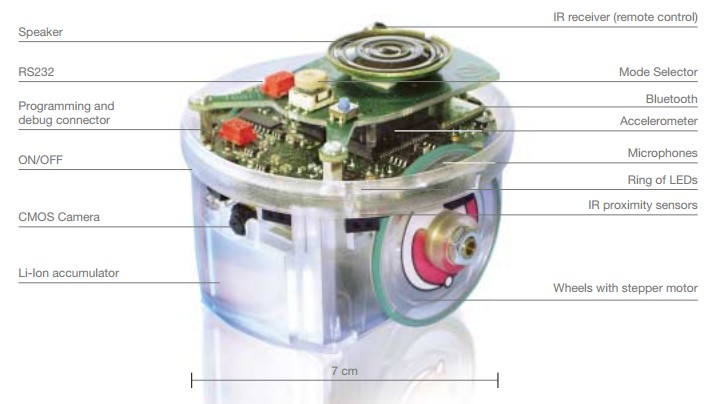
\includegraphics[scale=0.7]{img/e-puckTagged}

\section{Design Diagrams} \label{desSysDiag}
%use-case diagram
\begin{figure}[h!]
  \begin{tikzpicture}
    \begin{umlsystem}{Robot Functions}
      \umlusecase[x=0,y=0, name=useState]{Set State}
      \umlusecase[x=0,y=-1,name=useScan]{Scan Floor}
      \umlusecase[x=0,y=-2,name=useMove]{Move Around}
      \umlusecase[x=0,y=-3,name=useRotate]{Rotate}
      \umlusecase[x=0,y=-4,name=useSwap]{Swap Motor Strength}
      \umlusecase[x=0,y=-5,name=useConn]{Connect to other Robots} 
    \end{umlsystem}

    \umlactor[x=-6,y=-3.5]{User}
    \umlactor[x=6,y=-3.5]{Robot}

    \umlassoc{User}{useState}
    \umlassoc{Robot}{useState}
    \umlassoc{Robot}{useScan}
    \umlassoc{Robot}{useMove}
    \umlassoc{Robot}{useRotate}
    \umlassoc{Robot}{useSwap}
    \umlassoc{Robot}{useConn}
  \end{tikzpicture}
  \caption{Use Case Diagram for proposed software solution}
  \label{desSysUse}
\end{figure}

%Class Diagram
\begin{figure}[h!] 
  \begin{tikzpicture}
    \begin{umlpackage}{StiCo Algorithm}
      \umlclass[x=0,y=0]{Movement}{
        headMotorPower : short* \\ tailMotorPower : short* \\ tempPower : short*
      }{
        setMovementSpeed(short*, short*) : void \\ swapMovementSpeed(short*, 
        short*) : void
      }
      \umlclass[y=5]{Light}{
         lightStrength : short* \\ lightStorage : short**
       }{
         setLightStrength(short*) : void \\ scanLight(short**) : void
       }
       \umlclass[x=5,y=5]{Main}{}{}
       
       \umlimport{Main}{Movement}
       \umlimport{Main}{Light}
    \end{umlpackage}
  \end{tikzpicture}
  \caption{Class Diagram for StiCo Implementation}
  \label{desSysClassStiCo}
\end{figure}
\clearpage

%Traditional Design
%data dictionaries
\begin{landscape}
  \section{Data Dictionary}
  \begin{tabular}{| p{5cm} | p{4cm} | p{3cm} | p{6cm} |}
    \hline
    Attribute name & Description & Found in entity & Occurrence\\
    \hline
    lightStrength  & Stores current agent's light intensity & Light    &
    Whenever the agent needs to change light intensity              \\
    \hline
    lightStorage   & Stores localised light intensity       & Light    &
    When the agent scans the floor for localised messages           \\
    \hline
    headMotorPower & Stores left wheel movement strength    & Movement &
    When movement speed is modified or change in rotation direction \\
    \hline
    tailMotorPower & Stores right wheel movement strength   & Movement &
    When movement speed is modified or change in rotation direction \\
    \hline
    tempPower      & Stores headMotorPower                  & Movement &
    Used each time the robot needs to change rotational direction   \\
    \hline
    currentPos     & Stores agent's position                & Movement &
    Used during HybaCo execution.  Used to calculate moving decision\\
    \hline  
  \end{tabular}
\end{landscape}
\clearpage

\begin{figure}
  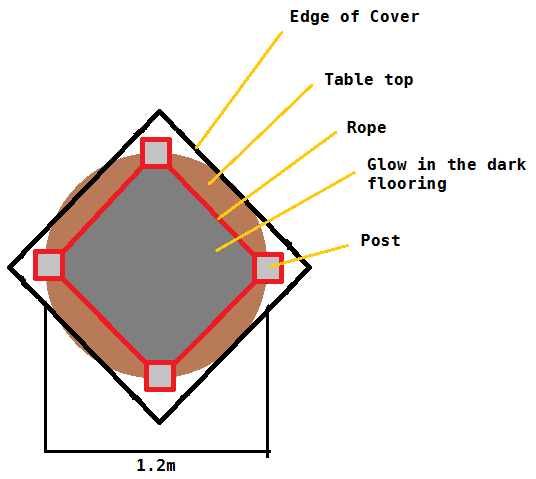
\includegraphics[scale=0.7]{img/ArenaTopDown.png}
  \caption{Top down view of the proposed dark room} \label{desSysTopImg}
\end{figure}
\begin{figure}
  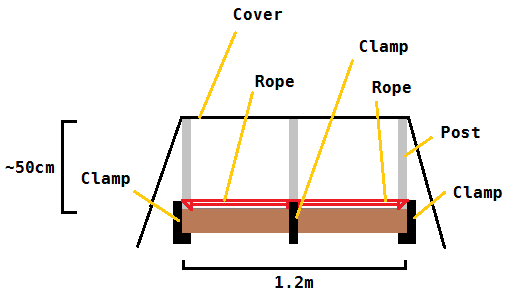
\includegraphics[scale=0.7]{img/ArenaSideView.png}
  \caption{Side view of the proposed dark room} \label{desSysSideImg}
\end{figure}
\clearpage

\section{Project Pseudo-code}
%pseudo code of main methods
\begin{algorithm}
  \caption{StiCo Algorithm\cite{Ranjbar-Sahraei2012Demo} }
  \label{desSysPseuStiCo}
  \begin{algorithmic}[1]
    \Require Each robot can deposit/detect pheromone trails \par
    \State Initialise: Choose circling direction (CW/CCW)
    \Loop
    \While{ (no pheromone is detected) }
    \State Circle around
    \State deposit Pheromone
    \EndWhile
    \If{ (interior sensor detects pheromone) }
    \State Reverse the circling direction
    \Else
    \While{ (pheromone is detected) }
    \State Rotate
    \EndWhile
    \EndIf
    \EndLoop
  \end{algorithmic}
\end{algorithm}

\section{Rope-length Algorithm}
\begin{algorithm}
  \caption{Rope Length Calculator (Measurements in centimetres) }
  \label{desSysRope}
  \begin{algorithmic}[1]
    \State $ Edge = 3(\sqrt{2(r^{2} ) } ) + 2 $
    \Comment Multiplying by 3 is due to tripling the rope over
    \State $ WrappedPost = (postPerimeter \times 2) + 2 $
    \Comment Trailing 2's are for securing the rope
    \State $ TotalRequiredRope = 4(Edge + WrappedPost) $
  \end{algorithmic}
\end{algorithm}
\clearpage

%\begin{landscape}
%Modified Gantt chart
\section{Gantt Chart}
\begin{ganttchart}[y unit chart=0.9cm]{1}{24}
  \gantttitle{2015}{12} \gantttitle{2016}{12} \\
  \gantttitlelist{1,...,12}{1} \gantttitlelist{1,...,12}{1} \\
  \ganttgroup{Req.}{1}{4} \\
  \ganttbar[name=reqRes]{Research}{1}{3} \\
  \ganttbar[name=reqWrite]{Req. Write Up}{4}{4} \\
  \ganttlink{reqRes}{reqWrite}
  
  \ganttgroup{Des.}{5}{8} \\
  \ganttbar[name=desArena]{ArenaBlueprints}{5}{7} \\
  \ganttbar[name=desAlSearch]{AlgorithmResearch}{5}{6} \\
  \ganttbar[name=desPseudo]{PseudoCode}{7}{7} \\
  \ganttmilestone[name=milDesFin]{Des. Content Finished}{7} \\
  \ganttbar[name=desWrite]{Des. Write Up}{8}{8} \\
  \ganttlink{desArena}{milDesFin}
  \ganttlink{desAlSearch}{desPseudo}
  \ganttlink{desPseudo}{milDesFin}
  \ganttlink{milDesFin}{desWrite}
  
  \ganttgroup{Imp.}{9}{20} \\
  \ganttbar[name=impArena]{Build Arena}{9}{11} \\
  \ganttbar[name=impFamiliar]{Coding Robot famil.}{10}{11} \\
  \ganttmilestone[name=milArenaFin]{Built Dark Room}{11} \\
  \ganttbar[name=impBasicCode]{Basic Code}{12}{14} \\
  \ganttbar[name=impAdvCode]{Advanced Code}{15}{17} \\
  \ganttmilestone[name=milCodeFin]{Finished Coding}{17} \\
  \ganttbar[name=impRefactor]{Refactor}{18}{18} \\
  \ganttbar[name=impWrite]{Imp. Write Up}{19}{20} \\
  \ganttlink{impArena}{milArenaFin}
  \ganttlink{impFamiliar}{milArenaFin}
  \ganttlink{milArenaFin}{impBasicCode}
  \ganttlink{impBasicCode}{impAdvCode}
  \ganttlink{impAdvCode}{milCodeFin}
  \ganttlink{milCodeFin}{impRefactor}
  \ganttlink{milCodeFin}{impWrite}
\end{ganttchart}
%\end{landscape}
\clearpage


\chapter{Realisation Code / Images}
\section{Code written for the Project (main.c)} \label{appendCode}
\lstinputlisting[language=C,breaklines=true]{roboCode/stico/main.c}

\section{Sound Based Testing in v-Rep} \label{appendSoundPics}
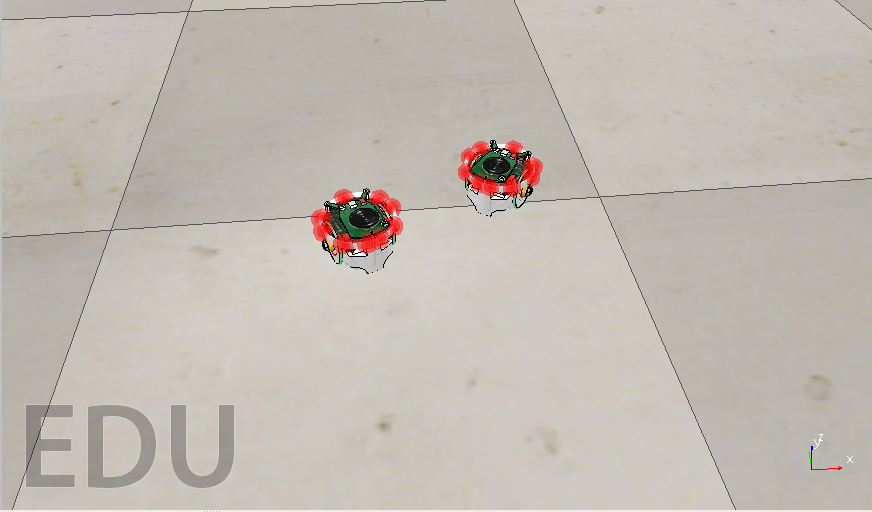
\includegraphics[scale=0.5]{img/puckSoundTest}
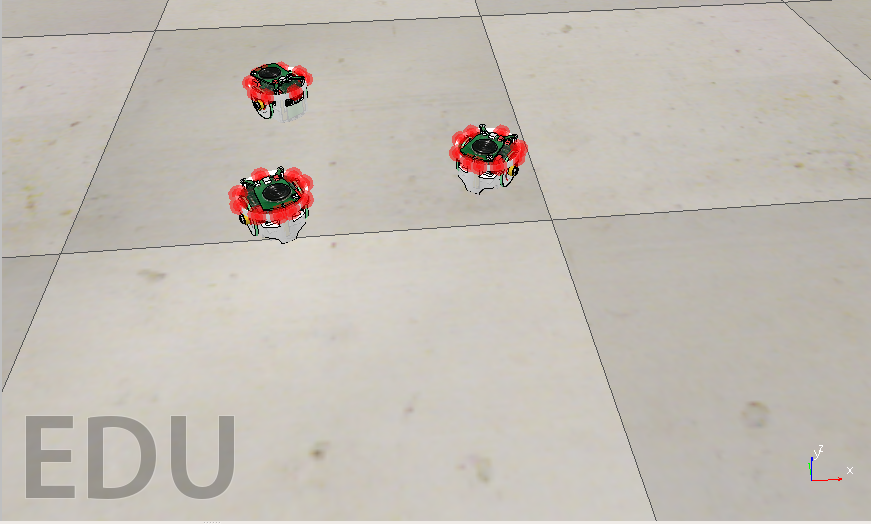
\includegraphics[scale=0.5]{img/puckSoundTest2}

\end{document}
